\section{ミニ2048}
本研究はミニ2048~\cite{YaKN22J}を研究対象として使用する.
% ミニ2048は,$3\times 3$ の盤面でプレイされることを除いて,確率的一人ゲーム{2048}と同じゲームである.

\subsection{ルール}

ミニ2048は,$3\times 3$ の盤面でプレイされる,確率的一人ゲーム{2048}の盤面縮小版である.
初期局面は盤面上に2つのタイル2(確率0.9)か4(確率0.1)の数字タイルがランダムに置かれた盤面からなる.

各局面において,プレイヤは上下左右いずれかの方向を選択する.
すると全ての数字タイルはその方向にできるだけ移動する.
移動した結果,2つの同じ数字のタイルが移動方向に衝突するとこれらは合体してその合計値のタイルとなり,
その合計値がスコアに加算される.合体してできたタイルは,同じターンでは別のタイルと合体することはない.
例えば,盤面の行が \verb*|2__|,\verb*|_22|,\verb*|224| であるとき,右を選択するとそれぞれ \verb*|__2|,\verb*|__4|,\verb*|_44| へと変化する.
その後,空白のマスのうちのランダムな1マスに2(確率0.9)か4(確率0.1)のタイルが置かれる.

プレイヤはいずれかのタイルが移動または衝突するような方向しか選択することができない.いずれの方向も選択できなくなるとゲームは終了する.
このゲームではできるだけ高い得点を獲得することが目標となる.
% このゲームの目標はゲームが終了する前に出来るだけ高得点を獲得することである.

\subsection{用語の導入}
通常の2048と同様にミニ2048における1ターンは,「移動・合体ステップ」と「新規タイルステップ」の2ステップからなる.これらステップの前後の状態を区別するため,以下の用語を導入する.
\begin{figure}[t]
  \centering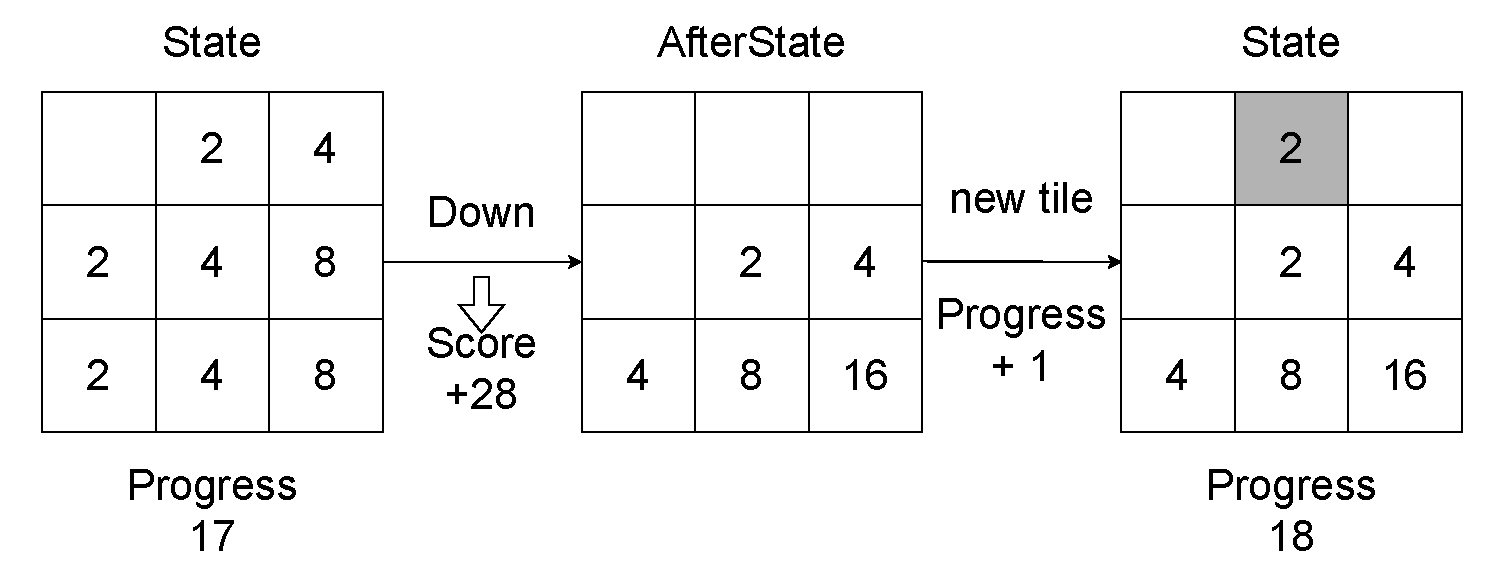
\includegraphics[width=.99\linewidth]{pdf/state_afterstate.drawio.pdf}
  \caption{state,afterstate,progressの例\cite{Terauchi25}}
  \label{afterstate}
 \end{figure}
\begin{description}
  \item[state] プレイヤが手を選択する盤面状態(とスコア)を\emph{state}と呼ぶ.
  \item[afterstate] プレイヤが手を選択してタイルが移動・合体した直後の盤面状態(とスコア)を\emph{afterstate}と呼ぶ.すなわち,afterstateは新規タイルが出現する前の盤面状態である.
 \end{description}

(通常の2048同様に)ミニ2048では,新しく出現するタイルはランダムに 2 か 4 の値をとる.そのため,単純にターン数をゲームの流さや進行度の指標に用いるには不都合がある.
この問題を解決するため,本研究では以下の指標を用いる.
\begin{description}
  % (\emph{時刻}~\cite{YaKa23J})これ抜いた
 \item[progress] タイルの値の合計値の半分を\emph{progress}~\cite{TeKM23}と呼ぶ.progress は,1ターンで1(新規タイルが2の場合)または2(新規タイルが4の場合)だけ増加する.
\end{description}

図\ref{afterstate}は,初期局面から始まるゲームの流れにおいて,state,afterstate,progress について図示したものである.


\subsection{完全解析とその結果}

ミニ2048は確率的一人ゲームであり,その完全解析とは各状態に対して期待スコア求めることである.
ミニ2048は,到達可能な状態数が $10^9$ 以下と小さいため,現実的な時間で完全解析ができる.
山下ら~\cite{YaKN22J}は,ミニ2048の完全解析に最初に取り組み,そこでは幅優先探索による状態列挙と,列挙した状態を用いる後退解析を行った.
また,著者ら~\cite{TeKM23}も完全解析の追試を行い,深さ優先探索による後退解析で,結果の正しさを確認した.

完全解析の結果について,重要なものを以下に示す.
初期状態のいずれかから到達可能な state の数は 48\,713\,519,afterstate の数は 31\,431\,374 である.
初期状態の期待スコアは,5\,468.49 である.
各 afterstate に対する期待スコアを格納したものを valueDB と呼ぶ.

完全解析で得られる valueDB を用いると,各局面において最適な手を選択するパーフェクトプレイヤを実現できる.
ただし,ミニ2048は確率的一人ゲームのため,決定的に最善手を選択するパーフェクトプレイヤであっても,ゲームごとに
プレイの結果は異なることに注意が必要である.
図\ref{pp-play}は,パーフェクトプレイヤが1万ゲームを行った際の,progress ごとの生存率とゲーム終了時のスコアを示している.
表\ref{pp-specific}は,パーフェクトプレイヤが256,512,1024タイルに到達したときの進捗状況,スコア,生存率を示している.
パーフェクトプレイヤでも,512タイルに到達した後,1024タイルに到達する前は,生存率が急激に低下することが分かる.
図\ref{pp-play}より,生存率が急激に下がるタイミングがいくつかある.
本研究では,そのような生存率が下がる部分を\emph{難易度の高い領域}と呼ぶ.
\begin{table}[t]
  \caption{Progress, score, and alive ratio of perfect player}
  \label{pp-specific}
  \centering\begin{tabular}{lrrr}
   \hline\hline
   Condition & ~~Progress & ~~Score~ & ~~~~Alive~~ \\
   \hline
  256-tile                          & 136~~~ & 1,750~ & 99.53\% \\
  512-tile                          & 263~~~ & 4,000~ & 73.84\% \\
  512-tile \& 256-tile              & 391~~~ & 5,750~ & 54.40\% \\
  512-tile \& 256-tile \& 128-tile  & 456~~~ & 6,500~ & 40.49\% \\
  1024-tile                         & 511~~~ & 9,000~ &  1.07\% \\
   \hline
\end{tabular}
\end{table}

\begin{figure}[t]
  \centering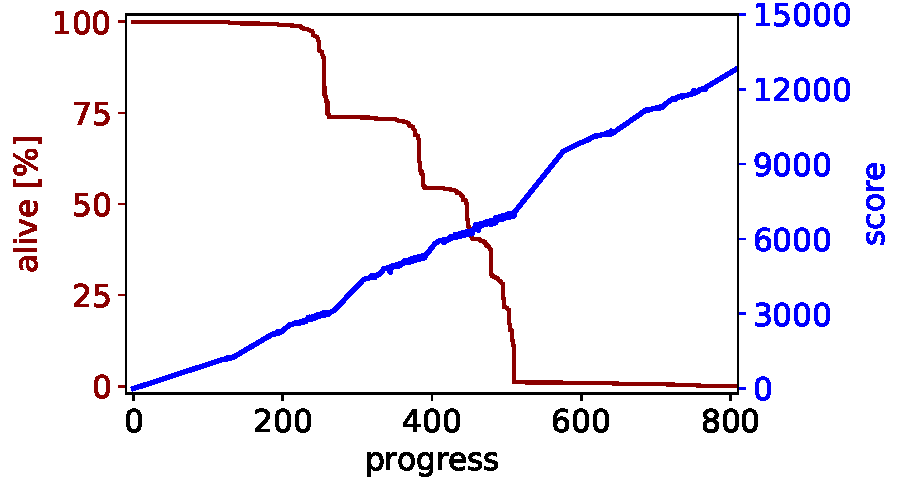
\includegraphics[width=\linewidth]{pdf/pp-play.pdf}
  \caption{パーフェクトプレイヤの生存率とスコア \cite{TeKM23}}
  \label{pp-play}
\end{figure}

% \section{パーフェクトプレイヤの結果を用いたミニ2048の分析}
% \subsection{プレイヤにノイズを加えた場合の平均得点の変化}

% 一般に,stateやafter stateの評価関数は完全に正確であるとは限らない.そこ,で評価関数が不正確な場合のスコアの変化を調査するため,valueDB にノイズを加えたシミュレーションを行った.
% ノイズは平均 0,分散 $\sigma^2$ の正規分布から生成し,標準偏差 $\sigma$ を 0 から 500 まで変化させた.
% このように変化させた valueDB を用いる貪欲プレイヤに 10,000 回のゲームをプレイさせ,その平均スコアを図~\ref{error_averagescore} に示す.

% % \begin{figure} 
% %   \centering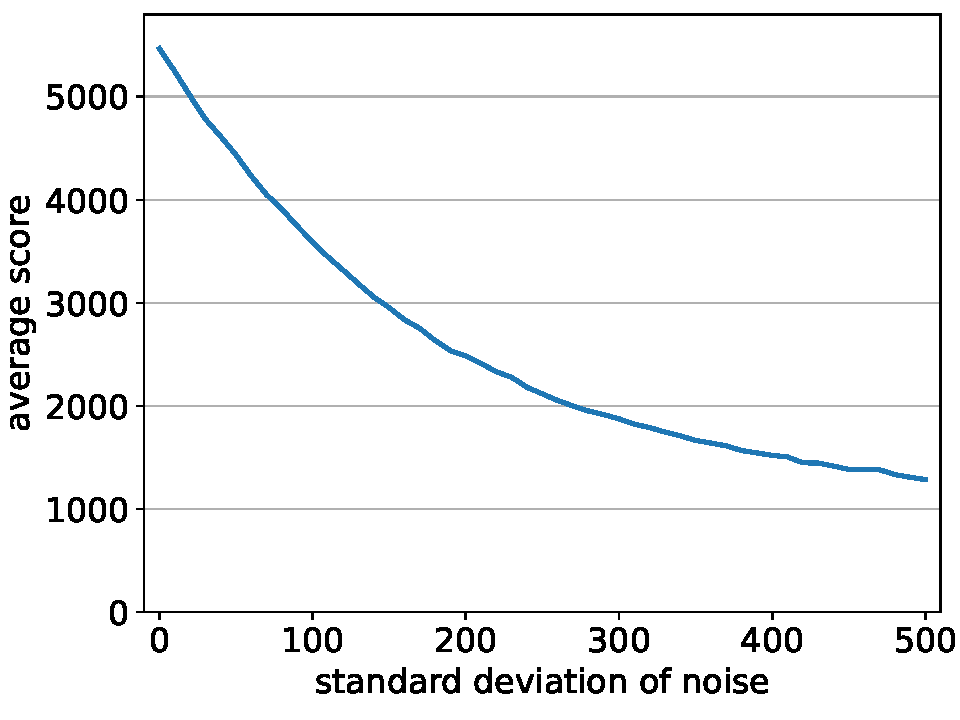
\includegraphics[height=0.40\textheight]{pdf/error_averagescore.pdf} 
% %   \caption{ノイズを加えたプレイヤの平均スコア} 
% %   \label{error_averagescore} 
% % \end{figure}

% 図~\ref{error_averagescore} より,標準偏差 $\sigma$ を大きくすると,平均スコアは単調に減少することが確認できる.
% 例えば,平均スコアが 5000,4000,3000,2000 となる $\sigma$ の値は,それぞれ $\sigma \approx 25, 75, 145, 270$ であった.
